\documentclass[11pt, titlepage]{article}
\usepackage{amsmath,amsthm,amssymb}
\usepackage{hyperref, pgf, tikz}
\usepackage{fancyhdr}
\usetikzlibrary{arrows}
\usepackage[margin=1.25in]{geometry}
\usepackage{graphicx}                     
\pagestyle{fancy}
\usepackage{array}
\usepackage{indentfirst}
%\usepackage{wrapfig}

\lhead{Lab \#3}
\rhead{\thepage}
\cfoot{}

\title{The RC Time Constant \\ \ \\ \large Lab \#3}
\author{Name: Avery Karlin \\ Partner: Jeffrey Zou}
\date{}
\begin{document}

\maketitle

\begin{center}
\LARGE The RC Time Constant
\end{center}

\section*{Objective}
The objective of the lab is to measure the time constant of an RC circuit based on the rate of charging and discharging.

\section*{Introduction}
Capacitors are defined by the equation $Q = CV$, such that the voltage of the capacitor is directly proportional to the charge, with the proportionality constant called the capacitance. Similar, resistor voltage is defined by Ohm's Law, such that $V = IR$. Thus, for a circuit purely with a resistor and a capacitor (RC circuit), the differential equation by Kirchoff's Voltage Law states that for charging (connected to the battery), $V_0 = \frac{Q}{C} + R\frac{dQ}{dt}$, and when discharging (disconnected from the battery), $0 = \frac{Q}{C} + r\frac{dQ}{dt}$. Thus, this can be solved to get an equation for charging, $V = V_0(1 - e^{\frac{-t}{RC}}) = V_0(1 - e^{\frac{-t}{\tau}}$ and for discharging, $V = V_0e^{\frac{-t}{RC}} = V_0e^{\frac{-t}{\tau}}$, where $\tau = RC$, called the time constant for an RC circuit.

These equations can be modified such that for charging, $-ln(\frac{V_0 - V}{V_0}) = -\frac{t}{RC}$ and for discharging, $-ln(\frac{V}{V_0}) = -\frac{t}{RC}$. Since the left-hand side here forms a constant term and the right is a constant multiplied by t, it forms a line with the slope equal to $\frac{-1}{RC}$.

\section*{Procedures and Results}

First, the power source is connected to a capacitor and then a variable resistor set to some value, joined back to the power source, with a voltmeter connected to the capacitor to measure the capacitor's charging voltage. After the power source is activated, it is timed with a stopwatch as it charges, recording the voltage as time increases, until the voltage of the capacitor is negligibly less than the battery, and it can't increase further. After, it is disconnected from the power source, such that the resistor is directly connected to the capacitor, such that it acts as the power source, discharging as voltage is lost through the resistor, recording the voltage as time increases again until it has only a negligible amount of voltage remaining. This is then repeated for a capacitor of a different capacitance.

\begin{figure}[h]
\centering
\hspace*{0cm}
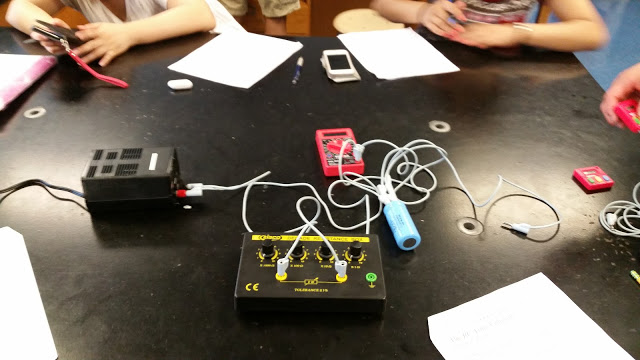
\includegraphics[scale=0.12, angle=90]{lab31.jpg}
\vspace*{0cm}
\end{figure}

\begin{figure}[h]
\centering
\hspace*{0cm}
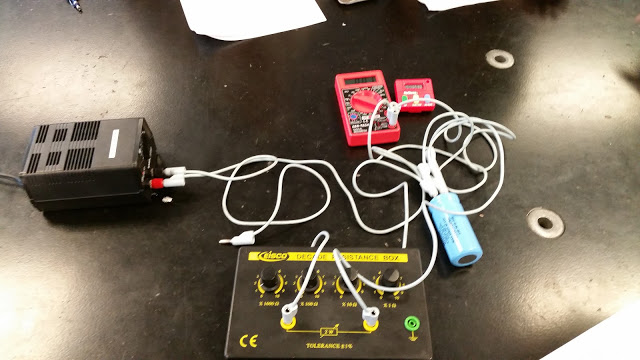
\includegraphics[scale=0.12, angle=270]{lab32.jpg}
\vspace*{0cm}
\end{figure}

\underline{Capacitor 1:}
\begin{center}
$$C = 5100 \mu F$$
$$R = 1350 \Omega$$
\begin{tabular}
{|m{9em}|m{9em}|m{9em}|}
\hline
Charging Time (s) & Charging Voltage (V) & Discharging Voltage (V) \\
\hline
0 & 0 & 8.87\\
\hline
4 & 3.48 & 5.48\\
\hline
8 & 5.47 & 3.37\\
\hline
12 & 6.8 & 2.12\\
\hline
16 & 7.53 & 1.43\\
\hline
20 & 8.06 & 0.9\\
\hline
24 & 8.31 & 0.6\\
\hline
28 & 8.51 & 0.38\\
\hline
32 & 8.63 & 0.26\\
\hline
36 & 8.72 & 0.17\\
\hline
40 & 8.77 & 0.12\\
\hline
\end{tabular}
\end{center}

\underline{Capacitor 2:}
\begin{center}
$$C = 4200 \mu F$$
$$R = 1350 \Omega$$
\begin{tabular}
{|m{9em}|m{9em}|m{9em}|}
\hline
Charging Time (s) & Charging Voltage (V) & Discharging Voltage (V) \\
\hline
0 & 0 & 8.91\\
\hline
4 & 5.18 & 4.74\\
\hline
8 & 7.16 & 2.30\\
\hline
12 & 7.84 & 1.13\\
\hline
16 & 8.26 & 0.6\\
\hline
20 & 8.60 & 0.33\\
\hline
24 & 8.75 & 0.16\\
\hline
28 & 8.81 & 0.10\\
\hline
32 & 8.87 & 0.06\\
\hline
36 & 8.89 & 0.03\\
\hline
40 & 8.90 & 0.02\\
\hline
\end{tabular}
\end{center}

\section*{Discussion}
Sample calculations for the non-measured data are as shown using the formulas found above:

$$R \text{(Voltmeter Interference, Small Resistor, Trial 1)} = \frac{V}{I - \frac{V}{R_V}} = \frac{2.6}{0.048 - \frac{2.6}{10^7}} = 54.16 \Omega$$
$$R \text{(Ammeter Interference, Small Resistor, Trial 1)} = \frac{V}{I} - R_A = \frac{2.6}{0.048} - 0.48 = 53.69 \Omega$$
$$R_{avg} \text{(Voltmeter Interference, Small Resistor)} = \frac{R_1 + R_2 + R_3}{3} = \frac{54.16 + 53.85 + 51.61}{3} = 53.21 \Omega$$
$$\text{Percent Error (Small Resistor, Voltmeter Interference)} = \frac{\text{$|$Expected - Actual$|$} * 100\%}{\text{Expected}} =$$\\$$\frac{|50.2 - 53.21| * 100\%}{53.21} = 5.66\%$$
$$R \text{(Wheatstone, Small Resistor, Trial 1)} = \frac{R_2R_K}{R_1} = \frac{12.8*50.2}{24.2} = 26.55 \Omega$$

\underline{Small Resistor:}
\begin{center}
\begin{tabular}
{|m{9em}|m{7em}|m{7em}|m{7em}|}
\hline
Rheostat Setting & 1 & 2 & 3 \\
\hline
Resistance, R $(\Omega)$ & 54.16 & 53.85 & 51.61\\
\hline
\end{tabular}
\\Average Resistance ($\Omega$) = 53.21
\\Percent Error = 5.66\%
\end{center}

\begin{center}
\begin{tabular}
{|m{9em}|m{7em}|m{7em}|m{7em}|}
\hline
Rheostat Setting & 1 & 2 & 3 \\
\hline
Resistance, R $(\Omega)$ & 53.69 & 53.37 & 49.52\\
\hline
\end{tabular}
\\Average Resistance ($\Omega$) = 52.19
\\Percent Error = 3.96\%
\end{center}

\underline{Large Resistor:}
\begin{center}
\begin{tabular}
{|m{9em}|m{7em}|m{7em}|m{7em}|}
\hline
Rheostat Setting & 1 & 2 & 3 \\
\hline
Resistance, R $(\Omega)$ & 78.79 & 79.31 & 79.17\\
\hline
\end{tabular}
\\Average Resistance ($\Omega$) = 79.09
\\Percent Error = 5.88\%
\end{center}

\begin{center}
\begin{tabular}
{|m{9em}|m{7em}|m{7em}|m{7em}|}
\hline
Rheostat Setting & 1 & 2 & 3 \\
\hline
Resistance, R $(\Omega)$ & 80.77 & 78.83 & 80.47\\
\hline
\end{tabular}
\\Average Resistance ($\Omega$) = 80.02
\\Percent Error = 7.12\%
\end{center}

\underline{Wheatstone Bridge:}
\begin{center}
\begin{tabular}
{|m{9em}|m{7em}|m{7em}|m{7em}|}
\hline
Trial & 1 & 2 & 3 \\
\hline
Resistance, R $(\Omega)$ & 26.55 & 26.87 & 25.6\\
\hline
\end{tabular}
\\Average Resistance $(\Omega)$ = 26.34
\\Percent Error = 2.9\%
\end{center}

\begin{center}
\begin{tabular}
{|m{9em}|m{7em}|m{7em}|m{7em}|}
\hline
Trial & 1 & 2 & 3 \\
\hline
Resistance, R $(\Omega)$ & 76.8 & 76.56 & 78.55 \\
\hline
\end{tabular}
\\Average Resistance $(\Omega)$ = 77.3
\\Percent Error = 3.48\%
\end{center}

The most likely cause of error is compounding loss of specificity due to the incorrect settings used on the multimeters. In addition, since the large resistors tend to have greater percent error than the other resistors, it indicates the measurement for that resistor's resistance may have been too low in some regard. Otherwise though, the overall percent error for each of the pieces of data was relatively low, such that it is mainly accurately done.

\section*{Conclusion}

The measured average resistance of the small resistor with the voltmeter needing to be accounted for, with an actual resistance of $50.2 \Omega$, was $53.21 \Omega$ with a percent error of 5.66\%. The measured average resistance of the small resistor with the ammeter needing to be accounted for, with an actual resistance of $50.2 \Omega$, was $52.19 \Omega$ with a percent error of 3.96\%. The measured average resistance of the large resistor with the voltmeter needing to be accounted for, with an actual resistance of $74.7 \Omega$, was $79.09 \Omega$ with a percent error of 5.88\%. The measured average resistance of the large resistor with the ammeter needing to be accounted for, with an actual resistance of $74.7 \Omega$, was $80.02 \Omega$ with a percent error of 7.12\%. The measured average resistance of the small resistor by the wheatstone bridge, with an actual resistance of $25.6 \Omega$, was $26.34 \Omega$ with a percent error of 2.9\%. The measured average resistance of the large resistor by the wheatstone bridge, with an actual resistance of $74.7 \Omega$, was $77.3 \Omega$ with a percent error of 3.48\%.

\end{document}
